% Auteur : Romain TESTUD
\begin{frame}{Les attaques}
    \begin{itemize}
        \item De nombreux cas d'attaque sur des CEX\footnotemark.
        \item Des sommes importantes sont concernés.
    \end{itemize}
    \begin{figure}
        \centering
        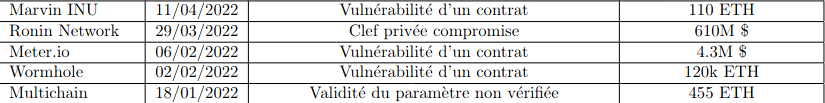
\includegraphics[scale = 0.45]{img/attaques.png}
        \label{fig:my_label2}
        %\caption{caption}
    \end{figure}
    \footnotetext{Centralised EXchange}
\end{frame}

\begin{frame}{Wormhole}
    Attaque sur le bridge entre Solana et Ethereum :
    \begin{itemize}
        \item Quelques heures après un correctif non déployé.
        \item Exploitation d'un défaut d'implémentation.
        \item La transaction de l'attaquant est signée par les gardiens.
        
    \end{itemize}
\end{frame}
\begin{frame}{Wormhole}
    \begin{block}{Fonctionnement du dépôt de jeton}
        \begin{itemize}
            \item Appel de plusieurs fonctions de vérification lors du dépôt.
            \begin{itemize}
                \item $complete\_wrapped$ $\Rightarrow$ 
                 $transfer\_message$
                 $\Rightarrow$  $post\_vaa$
                 $\Rightarrow$  $verify\_signature$
            \end{itemize}
            %\item Fonction complete\_wrapped appellée lors du mint de Wormhole ETH sur Solana
            %\item transfer\_message en paramètre : spécifie le token et combien doit être mint, signé par les gardiens
            %\item Contrat sur Solana, créé en utilisant la fonction post\_vaa qui vérifie la signature des gardiens
            %\item Appel a verify\_signature qui utilise un programme de Solana pour verifier les signatures
        \end{itemize}
        Erreur d'implémentation dans $verify\_signature$.
    \end{block}
\end{frame}

\begin{frame}{Wormhole}
    \begin{block}{$verify\_signature$ appelle un programme de vérification}
        \begin{itemize}
            \item $Sysvar: Instructions$ : Alias du programme.
            \item Vérification des signatures des gardiens.
            \item Il est possible d'utiliser d'une adresse différente.
        \end{itemize}  
    \end{block}
    \begin{figure}
        \centering
        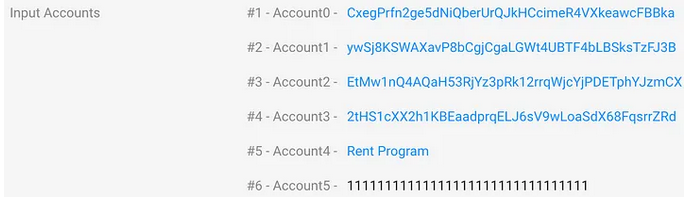
\includegraphics[scale = 0.3]{img/wormhole_img1.png}
    \end{figure}
\end{frame}

\begin{frame}{Wormhole}
    \begin{itemize}
        \item Adresse tierce entrée par l'attaquant.
        \item Validation de la transaction sans signature.
    \end{itemize}
        \begin{figure}
        \centering
        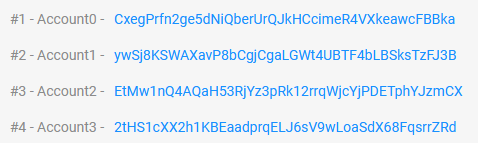
\includegraphics[scale = 0.7]{img/wormhole_img2.png}
    \end{figure}
\end{frame}



\begin{frame}{Nomad}
    \begin{itemize}
        \item Protocole d'échange entre blockchains.
        \item Utilisation de smart contracts.
        \item Erreur d'implémentation dans le contrat Réplica.
    \end{itemize}
    $\Rightarrow$ Possibilité de passer la vérification des messages.
\end{frame}

\begin{frame}{Nomad}
    \begin{block}{Fonctionnement de Nomad}
        \begin{itemize}
            \item Les messages ont des racines.
            \item Vérification de la racine lors de l'émission du message.
            \item Appel de la fonction process pour vérifier et envoyer le message.
        \end{itemize}
    \end{block}
    \pause
    \begin{block}{Vérification}
        \begin{itemize}
            \item $acceptableRoot$ : vérification de la validité de la racine du contrat.
        \end{itemize}
    \end{block}
\end{frame}

\begin{frame}{Nomad}
    \begin{block}{Défaut d'implémentation}
        \begin{itemize}
            \item La racine $0x00$ est valide.
            \item La racine par défaut des messages est $0x0$
        \end{itemize}
        $\Rightarrow$ Un message avec une racine nulle est donc par défaut valide.
    \end{block}
\end{frame}

\begin{frame}{Des solutions ?}
    \begin{itemize}
        \item Etablir des standards ?
        \item Supprimer le tiers de confiance ?
    \end{itemize}
    $\Rightarrow$ Vers le décentralisé
\end{frame}
